\subsection{Approach A——Morphology and HSV based Algorithm}
The pseudocode for the morphology and HSV based apple counting method is summarised in Algorithm~\ref{alg:morphological}. Taking the counting test dataset as an example, we first convert the images' colour space to Hue, Saturation, Value (HSV). We then apply inRange thresholding to highlight the foreground. Next, we break two slightly connected foreground regions with morphological opening and draw their contours. Finally, we count all contours with an area greater than $200$ and compare the number with the ground truth, if equal, the task is completed, otherwise it fails. The ratio of all successful cases to the total number of images is the precision. 

\begin{algorithm}[htb]
\label{alg:morphological}
\caption{Morphology and HSV based Algorithm} % 算法的名字
\hspace*{0.02in} {\bf Input:} counting test dataset\\% 算法的输入, \hspace*{0.02in}用来控制位置,\\ 换行
\hspace*{0.02in} {\bf Output:} precision % 算法的结果输出
\begin{algorithmic}[1]

\For{every image in the datasets} % For 语句,需要和EndFor对应
  \State HSV $\gets$ RGB
  \State inRange thresholding (mask)
  \If{$lower\ value \le src(x, y) \le higher\ value$} % If 语句,需要和EndIf对应
    \State $dst(x, y) = 255$
  \Else
    \State $dst(x, y) = 0$
  \EndIf
  \State opening
  \State find contours
  \For{every contour}
      \State calculate the area 
      \If{$area \ge 200$}
          \State $counter \gets counter + 1$
      \Else
          \State continue
      \EndIf
  \State compare counter to ground truth
  \If{$counter == ground\ truth$}
      \State True
  \Else
      \State False
  \EndIf
  \EndFor
\EndFor
\State \Return $precision = \frac{Number\ of\ 'True's}{Number\ of\ images}\times 100\%$
\end{algorithmic}
\end{algorithm}


\subsubsection{HSV}
Hue, Saturation, Value (HSV) is a colour space, commonly used in image processing, in which each colour can be expressed as three digits (Fig.~\ref{fig:HSV diagram}). Compared to RGB, HSV is closer to the perception of colour by human eyes and is therefore beneficial for the extraction of colour features. In the experiment, we identify the target object by setting the HSV range.

\begin{figure}[htb]
    \centering
    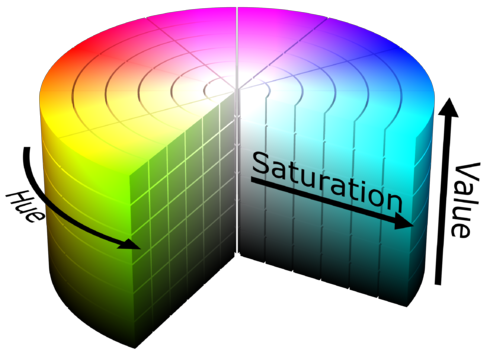
\includegraphics[width=0.35\textwidth]{images/HSV.png}
    \caption{Hue, Saturation, Value colour space (source: \url{https://upload.wikimedia.org/wikipedia})}
    \label{fig:HSV diagram}
\end{figure}

\subsubsection{InRange Thresholding}
InRange thresholding is an image thresholding method with the help of which we create binary images from HSV images, thus separating foreground from background~\citep{Nixon2020}. Specifically, when the source pixel value lies between the two given thresholds, it is assigned a value of 255 and the pixel values outside this range are assigned a value of 0. The expression is as follows:
\begin{equation}
    d(x, y) = \left\{\begin{matrix}
    &255& \quad if\ lower\ value\le s(x, y)\le higher\ value \\
    &0& \quad otherwise
    \end{matrix}\right.
\end{equation}

% \subsubsection{Median Filtering}

% \begin{equation}
%     g(x, y) = med\{f(x-k, y-l)\quad  k, l \in W\}
% \end{equation}

% \begin{figure}[htb]
%     \centering
%     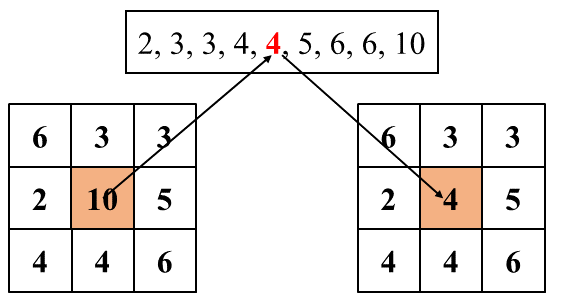
\includegraphics[width=0.4\textwidth]{images/median_filter.png}
%     \caption{Calculation principle of median filtering}
%     \label{fig:princinple of median filtering}
% \end{figure}

\subsubsection{Morphological Opening}
Opening, which is erosion followed by dilation, is used to separate two regions that are finely connected. Erosion and dilation are the two basic operations in morphological processing, on which all other morphological operations are built. The principle of the erosion is to calculate a local minimum in the region of the set kernel and replace the image pixels under the centroid with that value to eliminate the boundary pixel points of the connected regions so that the boundaries shrink inwards, the expression for which is~\citep{OpenCV2022}:
\begin{equation}
    d(x, y) = \eqnmarkbox[blue]{min}{min}_{(x', y')|pixel(x', y')\ne 0}\ s(x+x', y+y')
\end{equation}

where $d(x, y)$ is the destination pixel and the source pixel value ($s(x+x', y+y')$) is replaced by the smallest and non-zero pixel value in the neighbourhood. 

In contrast to erosion, the expansion operation calculates the maximum pixel value that overlaps the kernel and replaces the pixel at the centroid position with that value, resulting in an expansion of the bright region. The expression is~\citep{OpenCV2022}:
\begin{equation}
    d(x, y) = \eqnmarkbox[red]{max}{max}_{(x', y')|pixel(x', y')\ne 0}\ s(x+x', y+y')
\end{equation}

The outcome of the opening operation is shown in Fig.~\ref{fig:'i'}.

\begin{figure}[!ht]
    \centering
    \subfigure[Original 'i']{
\includegraphics[width=0.15\textwidth]{images/origin_i.png}}
    \subfigure[Eroded 'i']{
\includegraphics[width=0.15\textwidth]{images/eroded_i.png}}
    \subfigure[Dilated 'i']{
\includegraphics[width=0.15\textwidth]{images/dilated_i.png}}
    \caption{Eroded and dilated 'i' image~\citep{OpenCV2022}——(a)original 'i', (b) eroded 'i' and (c) dilated 'i'}
    \label{fig:'i'}
\end{figure}


\subsubsection{Contour Finding}
We adopt the Depth-First Search (DFS) algorithm to obtain the contours of the apples (Fig.~\ref{fig:DFS}). The principle is to start traversing down from the starting point and stop when there is no next node~\citep{Gross2003}. This is followed by traversing back to the previous node and continuing in the other direction until all nodes have been traversed.

\begin{figure}[htb]
    \centering
    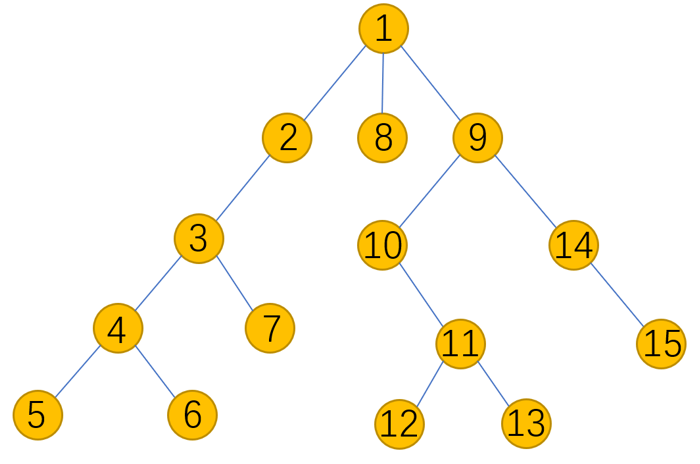
\includegraphics[width=0.4\textwidth]{images/Depth-first-treepng.png}
    \caption{Depth-first search algorithm}
    \label{fig:DFS}
\end{figure}

The advantage of the DFS algorithm is its low time complexity, unless a single route is unusually long. Still, its time complexity is much lower in magnitude than Canny and Sobel. Also, because of the size of the dataset, and the abundance of information in each image, the DFS algorithm is the logical choice.



\subsection{Approach B——Deep Learning}
The network structure of YOLOX (Fig.~\ref{fig:YoloX network structure}) consists of CSPDarknet, Feature Pyramid Network (FPN) and YOLO head. The CSPDarknet is the backbone feature extraction network of YOLOX~\citep{Ge2021}, which composes the extracted features as the input feature set. We acquire three feature layers, namely the effective feature layers, to construct the next network.

\begin{figure}[!ht]
    \centering
    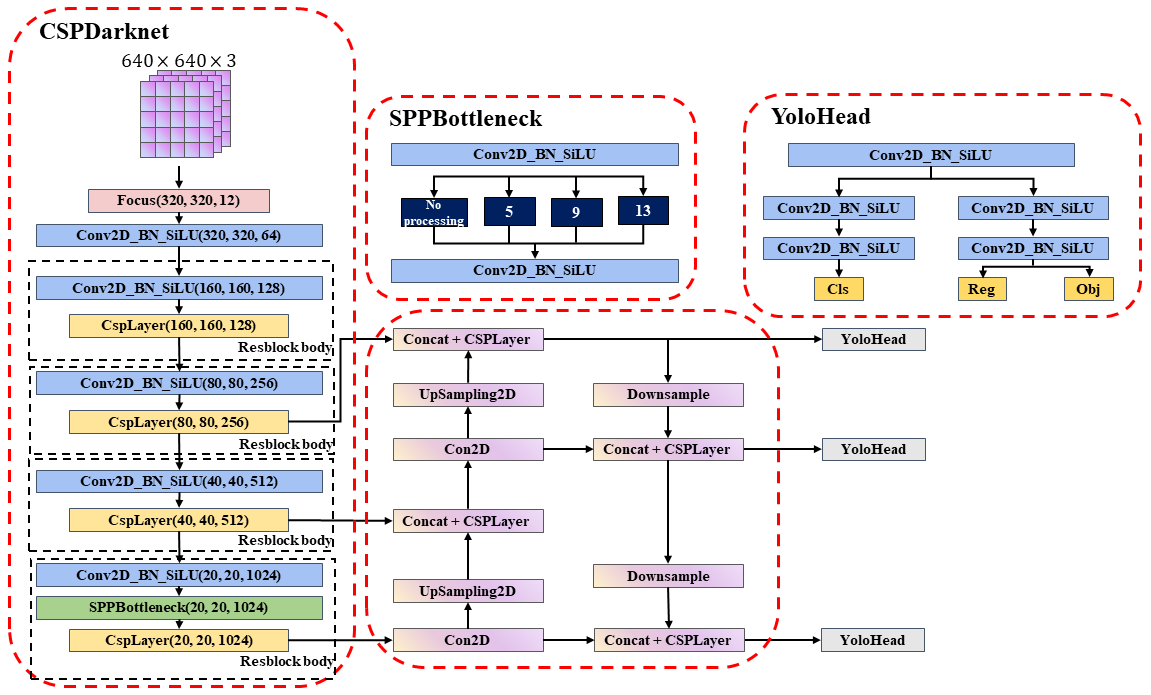
\includegraphics[width=1.1\textwidth]{images/Yolox_structure.png}
    \caption{YOLOX network structure}
    \label{fig:YoloX network structure}
\end{figure}

FPN extracts enhanced features, it fuses the effective feature layers to combine information at various scales. In FPN, we first upsample the features and then downsample them to achieve feature fusion. 

YOLO head is for classification and regression. We treat the previously obtained feature map as an ensemble of feature points, each of which has a number of features per channel. YOLO head determines whether a feature point corresponds to an object or not. Unlike previous versions of YOLO, the YOLO head in YOLOX is divided into two sections, implementing classification and regression respectively, which are integrated when predicting. In summary, the entire YOLOX workflow is: feature extraction, feature enhancement and predicting whether a feature point corresponds to an object or not.


\subsubsection{CSPDarknet}
YOLOX's backbone feature extraction network, CSPDarknet, has four outstanding attributes~\citep{Ge2021}.
\begin{enumerate}
    \item \textbf{The residual network.} The backbone of the residual convolution is the combination of a $1\times 1$ convolution and a $3\times 3$ convolution, with the residual edge portion incorporating the input and output of the backbone. By increasing the depth, the residual network can be optimised, thus improving the model's accuracy since the internal residual blocks are connected in a leap form to mitigate gradient disappearance. 
    
    \item \textbf{CSPNet.} The stacked residual blocks are dissected into two halves as shown in Fig.~\ref{fig:CSPnet}, with the backbone handling to continue to stack the residual blocks and the other part is similar to the residual edge and is joined to the end with little processing.
    
        \begin{figure}[htb]
            \centering
            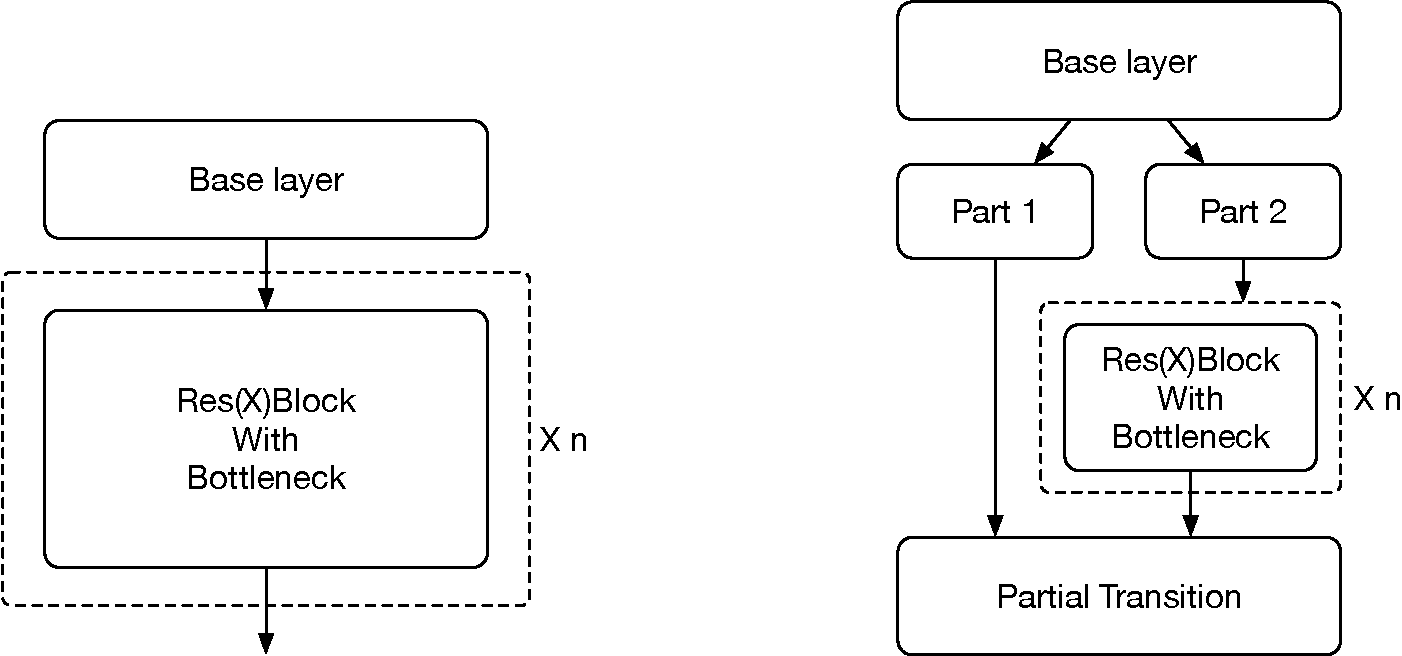
\includegraphics[width=0.6\textwidth]{images/Fig 4.7.pdf}
            \caption{CSPNet in the CSPDarknet}
            \label{fig:CSPnet}
        \end{figure}
    
    \item \textbf{Focus network structure.} As shown in Fig.~\ref{fig:Focus}, a value is taken every other pixel in an image to obtain four separate feature layers. Then stack the four separate feature layers thereby brings the width and height information into the channel information and the input channels are enlarged by four times (three channels → twelve channels).
    
        \begin{figure}[htb]
            \centering
            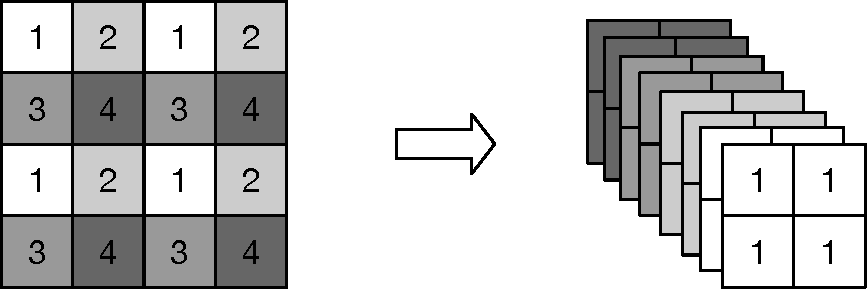
\includegraphics[width=0.5\textwidth]{images/Fig 4.8.pdf}
            \caption{Focus network structure}
            \label{fig:Focus}
        \end{figure}
    
    \item \textbf{SiLU activation function.} As shown in Fig.~\ref{fig:SiLU}, SiLU has the properties of being unbounded with a lower bound, smooth and non-monotonic~\citep{Elfwing2018}, and can be described as a smooth version of ReLU, which outperforms ReLU in deep models.
    
        \begin{figure}[htb]
            \centering
            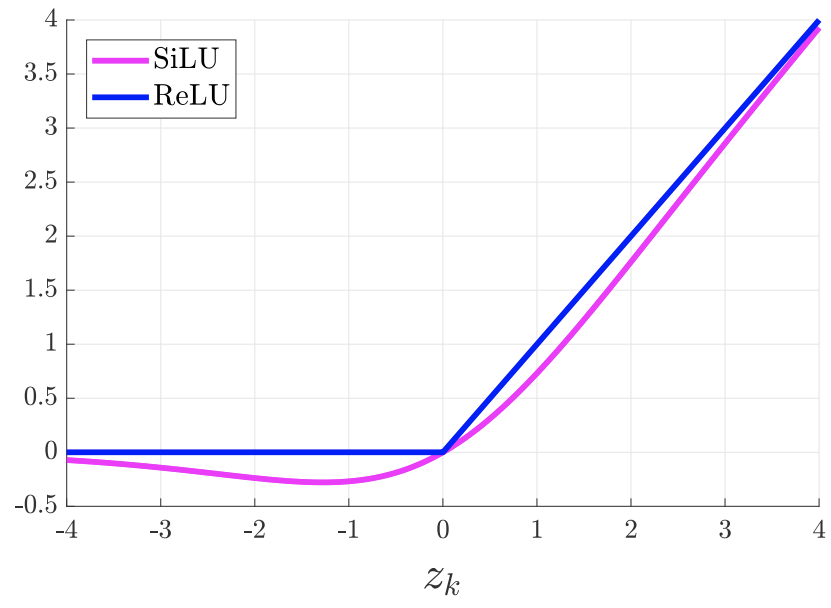
\includegraphics[width=0.5\textwidth]{images/SiLU.png}
            \caption{Curves of SiLU and ReLU activation functions~\citep{Elfwing2018}}
            \label{fig:SiLU}
        \end{figure}
    
\end{enumerate}


\subsubsection{Feature Pyramid Network}
In the feature utilisation phase, the three feature layers are situated in the middle, lower middle and bottom layers of the CSPDarknet (Fig.~\ref{fig:YoloX network structure}). When the input is $640\times 640\times 3$, the shapes of the three feature layers are: $feat_1 = 80\times 80\times 256$, $feat_2 = 40\times 40\times 512$ and $feat_3 = 20\times 20\times 1024$. The feature pyramid merges features with feature layers of different shapes to facilitate the extraction of more detailed features, and we build the FPN through the three effective feature layers.


\subsubsection{Decoupled YOLO Head}
We gain three enhanced features with dimensions of $80\times 80\times 256$, $40\times 40\times 512$ and $20\times 20\times 1024$ by FPN and pass them into YOLO head for prediction~\citep{Elfwing2018}. For each feature layer, we obtain three predictions, as shown in Fig.~\ref{fig:YOLO head}:
\begin{itemize}
    \item $Regression\ (h\times w\times 4)$——determines the regression parameters of the feature points, used to obtain the prediction bounding box.
    \item $Object\ (h\times w\times 1)$——determines if the feature point includes an object.
    \item $Classification\ (h\times w\times num\_classes)$——determines the class of the object contained in each feature point.
\end{itemize}

\begin{figure}[htb]
    \centering
    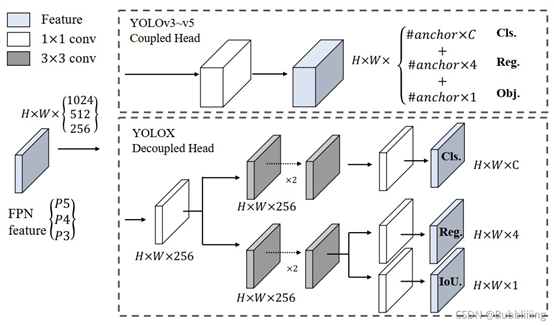
\includegraphics[width=0.65\textwidth]{images/YoloHead.png}
    \caption{Network structure of the YOLO heads within different versions of YOLO (source: \url{https://blog.csdn.net})}
    \label{fig:YOLO head}
\end{figure}

Stack the three predictions above, then the output of each feature layer is $h\times w\times (4 + 1 + num\_classes)$.


\subsubsection{Scoring Screening with Non-maximal Suppression}
We first find the prediction boxes with scores greater than the threshold function in the prediction outcomes. Subsequently, we apply non-maximal suppression to each class and sort them by score from highest to lowest. At last, we calculate the overlap of the highest scoring box with all other boxes and eliminate those with excessive overlap. The predictions without non-maximum suppression and with non-maximum suppression are shown in Fig.~\ref{fig:non-max suppression}.

\begin{figure}[htb]
    \centering
    \subfigure[Predictions before non-maximal suppression]{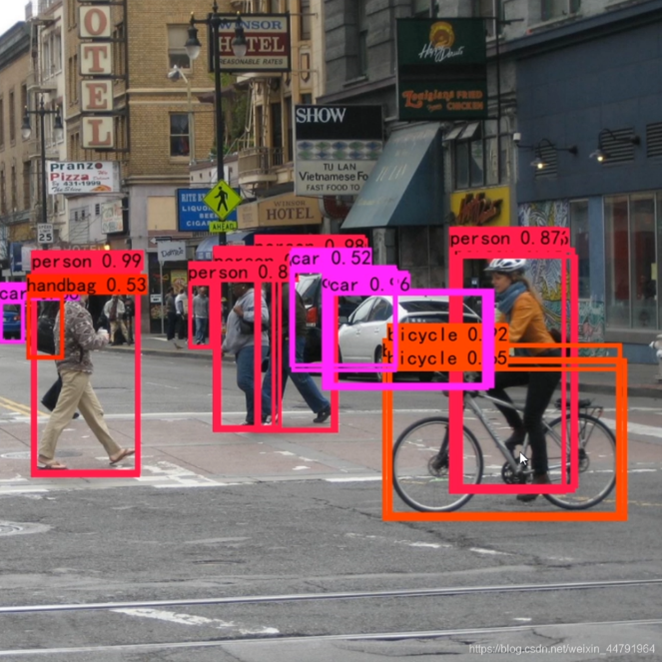
\includegraphics[width=0.4\textwidth]{images/non-max suppression_left.png}}
    \subfigure[Predictions after non-maximal suppression]{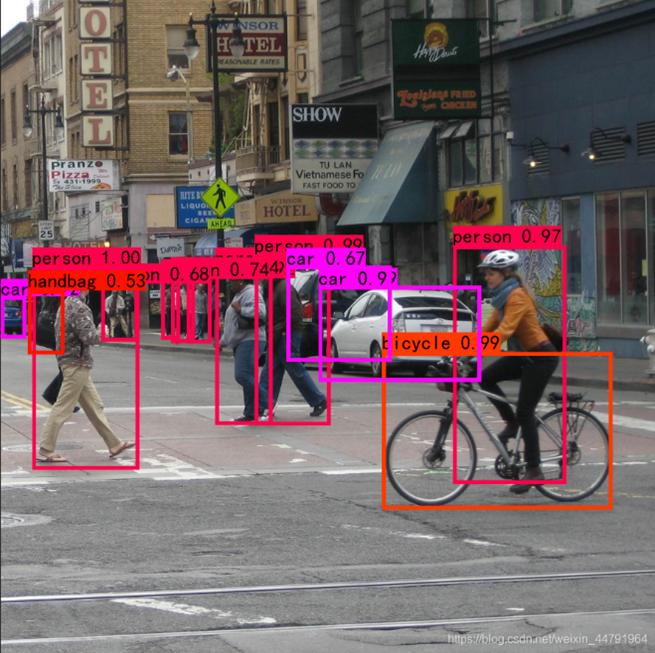
\includegraphics[width=0.4\textwidth]{images/non-max suppression_right.png}}
    \caption{Predictions before and after non-maximal suppression——(a) before and (b) after (source: \url{https://towardsdatascience.com})}
    \label{fig:non-max suppression}
\end{figure}
